
\chapter{Appendix}
\label{cha:appendix}

This chapter contains all the missing details from the previous chapters,
especially the proofs, experiment descriptions, and other relevant information.
This is done to ensure that the thesis is concise for all readers, and for
readers who are interested in low-level details they can refer to this chapter
as needed.

\section{Appendix for Chapter~\ref{CHA:ARS}}
\label{sec:append-chapt-refch}

\subsection{Proof of Theorem~\ref{thm:online_linear_regression}}
\label{sec:proofs_bandit}
\begin{proof}[Proof of Theorem~\ref{thm:online_linear_regression}]
%Result in Eq~\ref{eq:ogd} is directly from \cite{Zinkevich2003_ICML} with the fact that $\|w\|_2\leq\mathcal{W}$ and $\|\nabla_{w}\ell_t(w)\|_2\leq C\mathcal{X}$ to any $w$ and $t$.

To prove Eq.~\ref{eq:random_para} for Alg.~\ref{alg:random_search_OLR}, we use the proof techniques from \cite{flaxman2005online}. The proof is more simpler than the one in \cite{flaxman2005online} as we do not have to deal with shrinking and reshaping the predictor set ${\Theta}$.

Denote $u\sim \mathbb{B}_b$ as uniformly sampling $u$ from a $b$-dim unit ball, $u\sim\mathbb{S}_b$ as uniformly sampling $u$ from the $b$-dim unit sphere, and $\delta \in (0,1)$. Consider the loss function $\hat{c}_i(w_i) = \mathbb{E}_{v\sim \mathbb{B}_b}[c_i(\theta_i + \delta v)]$, which is a smoothed version of $c_i(w_i)$. It is shown in \cite{flaxman2005online} that the gradient of $\hat{c}_i$ with respect to $\theta$ is:
\begin{align*}
   &\nabla_{\theta}\hat{c}_i(\theta)|_{\theta = \theta_i} \\
   &= \frac{b}{\delta} \mathbb{E}_{u\sim\mathbb{S}_b}[c_i(\theta_i +\delta u)u]\\
   &= \frac{b}{\delta}\mathbb{E}_{u\sim \mathbb{S}_b}[((\theta_i +\delta u)^T s_i - a_i)^2 u].
\end{align*} Hence, the descent direction we take in Alg.~\ref{alg:random_search_OLR} is actually an unbiased estimate of $\nabla_{\theta}\hat{c}_i(\theta)|_{\theta=\theta_i}$. So Alg.~\ref{alg:random_search_OLR} can be considered as running OGD with an unbiased estimate of gradient on the sequence of loss $\hat{c}_i(\theta_i)$. It is not hard to show that for an unbiased estimate of $\nabla_{\theta}\hat{c}_i(\theta)|_{\theta=\theta_i}$ = $\frac{b}{\delta} ((\theta_i + \delta u)^T s_i - a_i)^2 u$, the norm is bounded as $b(C^2 + C_{s}^2)/\delta$. Now we can directly applying Lemma 3.1 from \cite{flaxman2005online}, to get:
\begin{align}
\label{eq:regret_on_surrogate}
   \mathbb{E}\left[\sum_{i=1}^T \hat{c}_i(\theta_i)\right] - \min_{\theta^\star\in{\Theta}}\sum_{i=1}^T \hat{c}_i(\theta^\star) \leq \frac{C_{\theta}b(C^2+C_{s}^2)}{\delta}\sqrt{T}.
\end{align} We can bound the difference between $\hat{c}_i(\theta)$ and ${c}_i(\theta)$ using the Lipschitiz continuous property of $c_i$:
\begin{align}
|\hat{c}_i(\theta) - c_i(\theta) | & = |\mathbb{E}_{v\sim \mathbb{B}_b}[c_i(\theta+\delta v) - c_i(\theta)]| \nonumber\\
&\leq \mathbb{E}_{v\sim \mathbb{B}_b}[|c_i(\theta+\delta v) - c_i(\theta)|] \leq L\delta.
\end{align} Substitute the above inequality back to Eq.~\ref{eq:regret_on_surrogate}, rearrange terms, we get:
\begin{align}
&\mathbb{E}\left[ \sum_{i=1}^T c_i(\theta_i)  \right]  - \min_{\theta^\star\in{\Theta}} \sum_{i=1}^T c_i(w^\star)\leq \frac{C_{\theta}b(C^2+C_{s}^2)}{\delta}\sqrt{T} + 2LT\delta.
\end{align} By setting $\delta = T^{-0.25}\sqrt{\frac{C_{\theta}b(C^2+C_{s}^2)}{2L}}$, we get:
\begin{align*}
   &\mathbb{E}\left[ \sum_{i=1}^T c_i(\theta_i)  \right]  - \min_{w^\star\in{\Theta}} \sum_{i=1}^T c_i(w^\star) \leq \sqrt{C_{\theta}b(C^2+C_{s}^2)L} T^{3/4}.
\end{align*}

To prove Eq.~\ref{eq:random_action} for Alg.~\ref{alg:random_search_action}, we follow the similar strategy in the proof of Alg.~\ref{alg:random_search_OLR}.

Denote $\epsilon \sim [-1,1]$ as uniformly sampling $\epsilon$ from the interval $[-1,1]$, $e\sim \{-1,1\}$ as uniformly sampling $e$ from the set containing $-1$ and $1$. Consider the loss function $\tilde{c}_i(\theta) = \mathbb{E}_{\epsilon\sim [-1,1]}[(\theta^T s_i + \delta \epsilon - a_i)^2]$. One can show that the gradient of $\tilde{c}_i(\theta)$ with respect to $\theta$ is:
\begin{align}
    \nabla_{\theta}\tilde{c}_i(\theta) = \frac{1}{\delta}\mathbb{E}_{e\sim \{-1,1\}}[e(\theta^{\top} s_i + \delta e - a_i)^2 s_i].
\end{align} As we can see that the descent direction we take in Alg.~\ref{alg:random_search_action} is actually an unbiased estimate of $\nabla_{\theta}\tilde{c}_i(\theta)|_{\theta=\theta_i}$. Hence Alg.~\ref{alg:random_search_action} can be considered as running OGD with unbiased estimates of gradients on the sequence of loss functions $\tilde{c}_i(\theta)$. For an unbiased estimate of the gradient, $\frac{1}{\delta} e(\theta_i^{\top} s_i +\delta e - a_i)^2 s_i$, its norm is bounded as $(C^2 + 1)C_{s}/\delta$. Note that different from Alg.~\ref{alg:random_search_OLR}, here the maximum norm of the unbiased gradient \emph{is independent of feature dimension $b$}. Now we apply Lemma 3.1 from \cite{flaxman2005online} on $\tilde{c}_i$, to get:
\begin{align}
\label{eq:tilde_random_action}
    \mathbb{E}\left[ \sum_{i=1}^T \tilde{c}_i(\theta_i)\right] - \min_{\theta^\star\in{\Theta}}\sum_{i=1}^T \tilde{c}_i(\theta^*) \leq \frac{C_{\theta}(C^2 + 1)C_{s}}{\delta}\sqrt{T}.
\end{align}
Again we can bound the difference between $\tilde{c}_i(\theta)$ and $c_i(\theta)$ for any $\theta$ using the fact that $(\hat{a}_i - a_i)^2$ is Lipschitz continuous with respect to prediction $\hat{a}_i$ with Lipschitz constant $C$:
\begin{align}
    |\tilde{c}_i(\theta) - c_i(\theta)| &= |\mathbb{E}_{\epsilon\sim [-1,1]} [(\theta^{\top} s_i + \delta\epsilon - a_i)^2 - (\theta^{\top} s_i - a_i)^2]|  \nonumber\\
    &\leq \mathbb{E}_{\epsilon\sim [-1,-1]}[C\delta |\epsilon|] \leq C\delta.
\end{align} Substitute the above inequality back to Eq.~\ref{eq:tilde_random_action}, rearrange terms:
\begin{align*}
    &\mathbb{E}\left[\sum_{i=1}^T \tilde{c}_i(\theta_i)\right] - \min_{\theta^\star\in{\Theta}}\sum_{i=1}^T \tilde{c}_i(\theta^*)\leq \frac{C_{\theta}(C^2+1)C_{s}}{\delta}\sqrt{T} + 2C\delta T.
\end{align*}
Set $\delta = T^{-0.25}\sqrt{\frac{C_{\theta}(C^2+1)C_{s}}{2C}}$, we get:
\begin{align*}
  &\mathbb{E}\left[\sum_{i=1}^T \tilde{c}_i(\theta_i)\right] - \min_{\theta^*\in{\Theta}}\sum_{i=1}^T \tilde{c}_i(\theta^*)\leq \sqrt{C_{\theta}(C^2+1)C_{s}C}T^{3/4}.
\end{align*}
\end{proof}




\subsection{Proof of Theorem~\ref{theorem:parameter-convergence}}
\label{sec:proofs_RL}

We first present some useful lemmas below.


Consider the smoothed objective given by $\hat{J}(\theta) =
\mathbb{E}_{v \sim \mathbb{B}_d}[J(\theta + \delta v)]$ where
$\mathbb{B}_d$ is the unit ball in $d$ dimensions and $\delta$ is a
positive constant. Using the assumptions stated in Section
\ref{sec:assumptions_parameter}, we obtain the following useful lemma:
\begin{lemma}
  \label{lemma:grad-diff-parameter}
  If the objective $J(\theta)$ satisfies the assumptions in Section
  \ref{sec:assumptions_parameter} and the smoothed objective
  $\hat{J}(\theta)$
  is as given above,
  %is given by $\hat{J}(\theta) = \mathbb{E}_{v \sim
  %  \mathbb{B}_d}[J(\theta + \delta v)]$ where $\delta > 0$ and
  %  $\mathbb{B}_d$ is the unit ball in $d$ dimensions
  then we have that
  \begin{enumerate}
  \item $\hat{J}(\theta)$ is also $G$-Lipschitz and $L$-smooth
  \item For all $\theta \in \mathbb{R}^d$, $\|\nabla_\theta J(\theta)
    - \nabla_\theta \hat{J}(\theta)\| \leq L\delta$
  \end{enumerate}
\end{lemma}



\begin{proof}[Proof of Lemma \ref{lemma:grad-diff-parameter}]
  Consider for any $\theta_1, \theta_2 \in \mathbb{R}^d$,
\begin{align*}
    |\hat{J}(\theta_1) - \hat{J}(\theta_2)| &= |\mathbb{E}_{v \sim \mathbb{B}_d}[J(\theta_1+\delta v) - J(\theta_2 + \delta v)]| \nonumber \\
    &\leq \mathbb{E}_{v \sim \mathbb{B}_d}[|J(\theta_1+\delta v) - J(\theta_2 + \delta v)|] \nonumber \\
    &\leq \mathbb{E}_{v \sim \mathbb{B}_d}[G\|\theta_1 - \theta_2\|] \nonumber \\
    &= G\|\theta_1 - \theta_2\|
\end{align*}
The above inequalities are due to the fact that expectation of absolute value is greater than absolute value of expectation, and the $G$-lipschitz assumption on $J(\theta)$. Thus, the smoothened loss function $\hat{J}(\theta)$ is also $G$-lipschitz. Similarly consider,
\begin{align*}
  \|\nabla_\theta\hat{J}&(\theta_1) - \nabla_\theta\hat{J}(\theta_2)\| \\
  &= \|\nabla_\theta \mathbb{E}_{v \sim \mathbb{B}_d}[J(\theta_1 + \delta v)] - \nabla_\theta \mathbb{E}_{v \sim \mathbb{B}_d}[J(\theta_2+\delta v)]\| \nonumber \\
    &= \|\mathbb{E}_{v \sim \mathbb{B}_d}[\nabla_\theta J(\theta_1+\delta v)
      - \nabla_\theta J(\theta_2 + \delta v)]\| \nonumber \\
    &\leq \mathbb{E}_{v \sim \mathbb{B}_d}[\|\nabla_\theta J(\theta_1+\delta
      v) - \nabla_\theta J(\theta_2 + \delta v)\|] \nonumber \\
    &\leq \mathbb{E}_{v \sim \mathbb{B}_d}[L\|\theta_1 - \theta_2\|] \nonumber \\
    &= L\|\theta_1 - \theta_2\|
\end{align*}
The above inequalities are due to the fact that expectation of norm is
greater than norm of expectation, and the $L$-smoothness assumption on
$J(\theta_1)$. We interchange the expectation and derivative using the
assumptions on $J(\theta_1)$ and the dominated convergence
theorem. Thus, the smoothened loss function $\hat{J}(\theta_1)$ is
also $L$-smooth.


We know,
  \begin{align*}
    \nabla_\theta \hat{J}(\theta) &= \nabla_\theta\mathbb{E}_{v \sim \mathbb{B}_d}[J(\theta +
                             \delta v)] \nonumber \\
    &= \mathbb{E}_{v \sim \mathbb{B}_d}[\nabla_\theta J(\theta + \delta v)]
  \end{align*}
  Note that the expectation and derivative can be interchanged using
  the dominated convergence theorem. Hence, we have
  \begin{align*}
    \|\nabla_\theta \hat{J}(\theta) - \nabla_\theta J(\theta)\| &= \|\mathbb{E}_{u \sim
                                                  \mathbb{B}_d}[\nabla_\theta
                                                  J(\theta + \delta v)]
                                                  - \nabla_\theta J(\theta)\|
                                                  \nonumber \\
                                                &\leq \mathbb{E}_{u \sim
                                                  \mathbb{B}_d}\|\nabla_\theta
                                                  J(\theta + \delta v) -
                                                  \nabla_\theta J(\theta)\|
                                                  \nonumber \\
                                                &\leq \mathbb{E}_{u
                                                  \sim \mathbb{B}_d}[L
                                                  ||\delta v||]
                                                  \nonumber \\
                                                &\leq L \delta
  \end{align*}
\end{proof}

The above lemma will be very useful later when we try to relate the
convergence rate for the smoothed objective and the true objective. It is shown in
\citep{flaxman2005online, agarwal2010optimal} that the gradient estimate $g_i$ is an
unbiased estimator of the gradient $\nabla_\theta
\hat{J}(\theta_i)$. Hence, Algorithm \ref{alg:random_search_parameter}
is performing SGD on the smoothed objective $\hat{J}(\theta)$. Using
this insight, we can use the convergence rate of SGD for nonconvex
functions to stationary points from \citep{ghadimi2013stochastic} which is given as
follows
\begin{lemma}[\citep{ghadimi2013stochastic}]
  \label{lemma:sgd-parameter}
  Consider running SGD on the objective $\hat{J}(\theta)$ that is
  $L$-smooth and $G$-Lipschitz for $T$ steps. Fix initial solution
  $\theta_0$ and denote $\Delta_0 = \hat{J}(\theta_0) -
  \hat{J}(\theta^*)$ where $\theta^*$ is the point at which
  $\hat{J}(\theta)$ attains global minimum. Also, assume that the
  gradient estimate $g_i$ is unbiased and has a bounded variance,
  i.e. for all $i$, $\mathbb{E}_i[\|g_i - \nabla_\theta
  \hat{J}(\theta_i)\|_2^2] \leq V \in \mathbb{R}^+$ where
  $\mathbb{E}_i$ denotes expectation with randomness only at iteration
  $i$ conditioned on history upto iteration $i-1$. Then we have,
  \begin{equation}
    %\label{eq:sgd-parameter}
    \frac{1}{T} \sum_{i=1}^T \mathbb{E}\|\nabla_\theta
    \hat{J}(\theta_i)\|_2^2 \leq \frac{2\sqrt{2\Delta_0L(V+G^2)}}{\sqrt{T}}
  \end{equation}
\end{lemma}
For completeness, we include a proof of the above lemma below.
\begin{proof}[Proof of Lemma \ref{lemma:sgd-parameter}]
  Denote $\xi_i = g_i - \nabla_\theta {\hat{J}}(\theta_i)$.  Note that $\mathbb{E}_{i} [\xi_i] =
0$ since the stochastic gradient $g_i$ is unbiased.
From  $\theta_{i+1} = \theta_i - \alpha g_i$, we have:
\begin{align*}
  \hat{J}(\theta_{i+1}) & = \hat{J}(\theta_{i} - \alpha g_i)\\
  &\leq\hat{J}(\theta_i) - \nabla_\theta \hat{J}(\theta_i)^{\top} (\alpha g_i) + \frac{L\alpha^2}{2}\| g_i\|_2^2  \\
    & = \hat{J}(\theta_i) - \alpha \nabla_\theta \hat{J}(\theta_i)^{\top} g_i + \frac{L\alpha^2}{2} \|\xi_i + \nabla_\theta \hat{J}(\theta_i)\|^2_2 \\
    & = \hat{J}(\theta_i) - \alpha \nabla_\theta
      \hat{J}(\theta_i)^{\top} g_i + \frac{L\alpha^2}{2}(\|\xi_i\|_2^2
  + 2\xi_i^{\top}\nabla_\theta \hat{J}(\theta_i) + \|\nabla_\theta \hat{J}(\theta_i)\|_2^2 )
\end{align*} The first inequality above is obtained since the loss
function $\hat{J}(\theta)$ is $L$-smooth. Adding $\mathbb{E}_i$ on both sides and using the fact that $\mathbb{E}_i [\xi_i] = 0$, we have:
\begin{align*}
    \mathbb{E}_i [\hat{J}(\theta_{i+1})] &= \hat{J}(\theta_i) - \alpha
                                           \|\nabla_\theta
                                           \hat{J}(\theta_i)\|_2^2  +\frac{L\alpha^2}{2}\left( \mathbb{E}_i [\|\xi_i\|_2^2] + \|\nabla_\theta \hat{J}(\theta_i)\|_2^2  \right)  \\
    &\leq \hat{J}(\theta_i) - \alpha \|\nabla_\theta
      \hat{J}(\theta_i)\|_2^2 + \frac{L\alpha^2}{2}\left( \mathbb{E}_i [\|\xi_i\|_2^2] + G^2  \right)
\end{align*}
where the inequality is due to the lipschitz assumption. Rearranging terms, we get:
\begin{align*}
    \alpha\|\nabla_\theta \hat{J}(\theta_i)\|_2^2 &= \hat{J}(\theta_i)
      - \mathbb{E}_i [\hat{J}(\theta_{i+1})] + \frac{L\alpha^2}{2} (\mathbb{E}_i [\|\xi_i\|_2^2] + G^2) \\
    & \leq \hat{J}(\theta_i) - \mathbb{E}_i[ \hat{J}(\theta_{i+1})] + \frac{L\alpha^2}{2} (V + G^2)
\end{align*}
Sum over from time step $1$ to $T$, we get:
\begin{align*}
    \alpha \sum_{t=1}^T \mathbb{E}\|\nabla_\theta
  \hat{J}(\theta_i)\|_2^2 &\leq \mathbb{E} [\hat{J}(\theta_0) -
                            \hat{J}(\theta_T)] + \frac{LT\alpha^2}{2}(V+G^2)
\end{align*} Divide $\alpha$  on both sides, we get:
\begin{align*}
    \sum_{t=1}^{T} \mathbb{E}&\|\nabla_\theta \hat{J}(\theta_i)\|_2^2 \leq \frac{1}{\alpha} \mathbb{E}[\hat{J}(\theta_0) - \hat{J}(\theta_T)] + {LT\alpha} (V+G^2) \\
    & \leq \frac{1}{\alpha} \mathbb{E}[\hat{J}(\theta_0) - \hat{J}(\theta^*)] + {LT\alpha} (V+G^2)  \\
    & = \frac{1}{\alpha} \Delta_0 + {LT\alpha} (V+G^2)  \\
    & \leq \sqrt{\frac{\Delta_0LT(V+G^2)}{2}} + \sqrt{2\Delta_0
      LT(V+G^2)} \\
      &\leq 2\sqrt{2\Delta_0 LT(V+G^2)}
\end{align*} with $\alpha = \sqrt{\frac{2\Delta_0}{LT(V+G^2)}}$.
Hence, we have:
\begin{align*}
    \frac{1}{T}\sum_{t=1}^T\mathbb{E}\|\nabla_\theta \hat{J}(\theta_i)\|_2^2 \leq \frac{2\sqrt{2\Delta_0 L(V+G^2)}}{\sqrt{T}}
\end{align*}
\end{proof}



The above lemma is useful as it gives us the following result:
\begin{align}
  \label{eq:stationary-point}
  \min_{1 \leq i \leq T} \mathbb{E}\|\nabla_\theta\hat{J}(\theta_i)\|_2^2 &\leq \frac{1}{T} \sum_{i=1}^T \mathbb{E}\|\nabla_\theta
                                                               \hat{J}(\theta_i)\|_2^2
                                                               \nonumber
  \\
                                                             &\leq \frac{2\sqrt{2\Delta_0L(V+G^2)}}{\sqrt{T}}
\end{align}
since the minimum is always less than the average. We have then that
using SGD to minimize a nonconvex objective finds a $\theta_i$ that is
`almost' a stationary point in bounded number of steps provided the
stochastic gradient estimate has bounded variance.

We now show that the gradient estimate $g_i$ used in Algorithm
\ref{alg:random_search_parameter} indeed has a bounded variance. Observe that
the estimate $g_i$ in the algorithm is a two-point estimate, which
should have substantially less variance than one-point
estimates \citep{agarwal2010optimal}. However, the two evaluations, resulting in $J_i^+$ and
$J_i^-$, have different independent noise. This is due to the
fact that in policy search, stochasticity arises from the
environment and cannot be controlled and we cannot obtain the
significant variance reduction that is typical of two-point
estimators. The following lemma quantifies the bound on the variance of
gradient estimate $g_i$:
\begin{lemma}
\label{lemma:grad-variance-parameter}
  Consider a smoothed objective $\hat{J}(\theta) = \mathbb{E}_{v \sim
    \mathbb{B}_d}[J(\theta + \delta v)]$ where $\mathbb{B}_d$ is the
  unit ball in $d$ dimensions, $\delta > 0$ is a scalar and the true
  objective $J(\theta)$ is $G$-lipschitz. Given gradient estimate $g_i
  = \frac{d(J_i^+ - J_i^-)}{2\delta}u$ where $u$ is sampled uniformly
  from a unit sphere $\mathbb{S}_d$ in $d$ dimensions, $J^+_i =
  J(\theta_i + \delta u) + \eta^+_i$ and $J_i^- = J(\theta - \delta u)
  + \eta_i^-$ for zero mean random i.i.d noises $\eta_i^+, \eta_i^-$, we have
  \begin{equation}
    \label{eq:grad-variance-parameter}
    \mathbb{E}_i[\|g_i - \nabla_\theta \hat{J}(\theta_i)\|_2^2] \leq
    2d^2G^2 + 2\frac{d^2\sigma^2}{\delta^2}
  \end{equation}
  where {$\sigma^2$ is the variance of the random noise $\eta$.}
\end{lemma}


\begin{proof}[Proof of Lemma \ref{lemma:grad-variance-parameter}]
  From \cite{shamir2017optimal}, we know that $g_i$ is an unbiased estimate of the gradient of $\hat{J}(\theta_i)$, i.e. $\mathbb{E}_{u_i \sim \mathbb{S}_d}[g_i] = \nabla\hat{J}(\theta_i)$. Thus, we have
\begin{align*}
    \mathbb{E}_{u_i \sim \mathbb{S}_d}&\|g_i -
      \nabla\hat{J}(\theta_i)\|^2 \\
      &= \mathbb{E}_{u_i \sim \mathbb{S}_d}[\|g_i\|^2 + \|\nabla \hat{J}(\theta)_i\|^2 - 2g_i^T\nabla \hat{J}(\theta_i)] \\
    &= \mathbb{E}_{u_i \sim \mathbb{S}_d}\|g_i\|^2 + \|\nabla \hat{J}(\theta_i)\|^2 - 2\|\nabla \hat{J}(\theta_i)\|^2 \\
    &= \mathbb{E}_{u_i \sim \mathbb{S}_d}\|g_i\|^2 - \|\nabla \hat{J}(\theta_i)\|^2 \\
    &\leq \mathbb{E}_{u_i \sim \mathbb{S}_d}\|g_i\|^2 \\
    &= \frac{d^2}{4\delta^2}\mathbb{E}_{u_i \sim
      \mathbb{S}_d}\|(J(\theta_i + \delta u_i) - J(\theta_i - \delta
      u_i) + (\eta_i^+ - \eta_i^-))u_i\|^2 \\
  &\leq \frac{d^2}{2\delta^2}[\mathbb{E}_{u_i \sim \mathbb{S}_d}\|(J(\theta_i + \delta u_i) - J(\theta_i - \delta
    u_i)u_i\|_2^2 + \mathbb{E}_{u_i \sim \mathbb{S}_d}\|(\eta_i^+ -
    \eta_i^-))u_i\|^2] \\
    &\leq \frac{d^2}{2\delta^2}[\mathbb{E}_{u_i \sim \mathbb{S}_d}
      4G^2\delta^2 \|u_i\|^2 +  4\mathbb{E}_{u_i \sim
      \mathbb{S}_d}\|\eta_i^+\|_2^2 \|u_i\|_2^2]\\
    &= 2d^2G^2  + 2\frac{d^2\sigma^2}{\delta^2}
\end{align*}
where the second inequality is true as $\|a+b\|_2^2 \leq 2(\|a\|_2^2 +
\|b\|_2^2)$ and the last inequality is due to the Lipschitz assumption
on $J(\theta)$.
\end{proof}

We are ready to prove Theorem~\ref{theorem:parameter-convergence}.
\begin{proof}[Proof of Theorem \ref{theorem:parameter-convergence}]
  Fix initial solution $\theta_0$ and denote $\Delta_0 =
  \hat{J}(\theta_0) - \hat{J}(\theta^*)$ where $\hat{J}(\theta)$ is
  the smoothed objective and $\theta^*$ is the point at which
  $\hat{J}(\theta)$  attains global minimum.
  Since the gradient estimate $g_i$ used in Algorithm
  \ref{alg:random_search_parameter} is an unbiased estimate of the
  gradient $\nabla_\theta \hat{J}(\theta_i)$, we know that Algorithm
  \ref{alg:random_search_parameter} performs SGD on the smoothed
  objective. Moreover, from Lemma \ref{lemma:grad-variance-parameter},
  we know that the variance of the gradient estimate $g_i$ is
  bounded. Hence, we can use Lemma \ref{lemma:sgd-parameter} on the
  smoothed objective $\hat{J}(\theta)$ to get
  \begin{align}
    \label{eq:sgd-parameter}
    \frac{1}{T} \sum_{i=1}^T \mathbb{E}\|\nabla_\theta
    \hat{J}(\theta_i)\|_2^2 \leq \frac{2\sqrt{2\Delta_0L(V+G^2)}}{\sqrt{T}}
  \end{align}
  where $V \leq 2d^2G^2 + 2\frac{d^2\sigma^2}{\delta^2}$ (from Lemma
  \ref{lemma:grad-variance-parameter}). We can relate $\nabla_\theta
  \hat{J}(\theta)$ and $\nabla_\theta J(\theta)$ - the quantity that
  we ultimately care about, as follows:
  \begin{align*}
    \frac{1}{T} &\sum_{i=1}^T \mathbb{E}\|\nabla_\theta
    J(\theta_i)\|_2^2\\
    &= \frac{1}{T} \sum_{i=1}^T
                        \mathbb{E}\|\nabla_\theta J(\theta_i) -
                        \nabla_\theta \hat{J}(\theta_i) +
      \nabla_\theta \hat{J}(\theta_i)\|_2^2 \\
    &\leq \frac{2}{T} \sum_{i=1}^T \mathbb{E}\|\nabla_\theta J(\theta_i) -
                        \nabla_\theta \hat{J}(\theta_i)\|_2^2 + \mathbb{E}\|\nabla_\theta \hat{J}(\theta_i)\|_2^2
  \end{align*}
  We can use Lemma \ref{lemma:grad-diff-parameter} to bound the first
  term and Equation \ref{eq:sgd-parameter} to bound the second
  term. Thus, we have
  \begin{align*}
    \frac{1}{T} \sum_{i=1}^T \mathbb{E}\|\nabla_\theta
    J(\theta_i)\|_2^2 \leq \frac{2}{T}[TL^2\delta^2 + 2\sqrt{2\Delta_0L(V+G^2)T}]
  \end{align*}
  Substituting the bound for $V$ from Lemma
  \ref{lemma:grad-variance-parameter}, using the inequality
  $\sqrt{a+b} \leq \sqrt{a} + \sqrt{b}$ for $a, b \in \mathbb{R}^+$,
  optimizing over $\delta$, and using $\Delta_0 \leq \Qbound$ we get
  \begin{equation*}
    \frac{1}{T} \sum_{i=1}^T \mathbb{E}\|\nabla_\theta
    J(\theta_i)\|_2^2 \leq \mathcal{O}(\Qbound^{\frac{1}{2}}dT^{\frac{-1}{2}} + \Qbound^{\frac{1}{3}}d^{\frac{2}{3}}T^{\frac{-1}{3}}\sigma)
  \end{equation*}
\end{proof}

\subsection{Proof of Theorem~\ref{theorem:action-convergence}}
\label{sec:proof-action-convergence}

The bound on the bias of the gradient estimate is given
by the following lemma:
\begin{lemma}
  \label{lemma:bias-bound-action}
  If the assumptions in Section \ref{sec:assumptions_action} are
  satisfied, then for  the gradient estimate $g_i$ used in Algorithm
  \ref{alg:random_search_action} and the gradient of the objective
  $J(\theta)$ given in equation \ref{eq:dpg-gradient}, we have
  \begin{equation}
    \label{eq:bias-bound-action}
    \|\mathbb{E}[g_i] - \nabla_\theta J(\theta_i)\| \leq KUH\delta
  \end{equation}
\end{lemma}


\begin{proof}[Proof of Lemma \ref{lemma:bias-bound-action}]
  To prove that the bias is bounded, let's consider for any $i$
  \begin{align*}
      &\|\mathbb{E}[g_i] - \nabla_\theta J(\theta_i)\|_2 = \|\sum_{t=0}^{H-1} \mathbb{E}_{s_t\sim
        d_{\pi_{\theta_i}}^t}[\nabla_\theta \pi(\theta_i, s_t) \nabla_a (\mathbb{E}_{v \sim \mathbb{B}_p}
        Q_{\pi_{\theta_i}}^t(s_t, \pi(\theta_i, s_t) + \delta v) -
          Q_{\pi_{\theta_i}}^t(s_t, \pi(\theta_i, s_t)))]\|_2 \\
    &\leq \sum_{t=0}^{H-1} \mathbb{E}_{s_t\sim d_{\pi_{\theta_i}}^t, v
      \sim \mathbb{B}_p}\|\nabla_\theta \pi(\theta_i, s_t)\|_2 \|[\nabla_a
      Q_{\pi_{\theta_i}}^t(s_t, \pi(\theta_i, s_t) + \delta v) -
      \nabla_a Q_{\pi_{\theta_i}}^t(s_t, \pi(\theta_i, s_t))]\|_2 \\
    &\leq \sum_{t=0}^{H-1} KU\delta \mathbb{E}_{v \sim
      \mathbb{B}_p}\|v\|_2 \\
    &\leq KUH\delta
  \end{align*}
  The first inequality above is obtained by using the fact that
  $\|\mathbb{E}[X]\|_2 \leq \mathbb{E}\|X\|_2$, and the second
  inequality using the $K$-lipschitz assumption on $\pi(\theta, s)$
  and $U$-smooth assumption on $Q_{\pi_\theta}^t(s, a)$ in $a$. Also,
  observe that we interchanged the derivative and expectation above by
  using the assumptions on $Q_{\pi_\theta}^t$ as stated in Section
  \ref{sec:assumptions_action}.
\end{proof}

We will now show that the gradient estimate $g_i$ used in Algorithm
\ref{alg:random_search_action} has a bounded variance. Note that the
gradient estimate constructed in Algorithm
\ref{alg:random_search_action} is a one-point estimate, unlike policy
search in parameter space where we had a two-point estimate. Thus, the variance would be higher and the bound
on the variance of such a one-point estimate is given below
\begin{lemma}
  \label{lemma:grad-variance-action}
  Given a gradient estimate $g_i$ as shown in Algorithm
  \ref{alg:random_search_action}, the variance of the estimate can be
  bounded as
  \begin{equation}
    \label{eq:grad-variance-action}
    \mathbb{E}\|g_i - \mathbb{E}[g_i]\|_2^2 \leq
    \frac{2H^2p^2K^2}{\delta^2} ((\Qbound + W\delta)^2 + \sigma^2)
  \end{equation}
  where $\sigma^2$ is the variance of the random noise $\tilde{\eta}$.
\end{lemma}



\begin{proof}[Proof of Lemma \ref{lemma:grad-variance-action}]
  To bound the variance of the gradient estimate $g_i$ in Algorithm
  \ref{alg:random_search_action}, lets consider
  \begin{align*}
    &\mathbb{E}_i\|g_i - \mathbb{E}[g_i]\|_2^2 = \mathbb{E}_i\|g_i\|_2^2 -
                                              \|\mathbb{E}_i[g_i]\|_2^2
                                            \leq \mathbb{E}_i\|g_i\|_2^2 \\
    &= \frac{H^2p^2}{\delta^2} \mathbb{E}_i\|\nabla_\theta
      \pi(\theta_i, s_t)
    (Q_{\pi_{\theta_i}}^t(s_t, \pi(\theta_i, s_t)
      + \delta u) + \tilde{\eta}_i) u\|_2^2 \\
    &\leq \frac{K^2p^2H^2}{\delta^2} \mathbb{E}_{i}\|Q_{\pi_{\theta_i}}^t(s_t, \pi(\theta_i,
      s_t) + \delta u)u + \tilde{\eta}_iu\|_2^2
  \end{align*}
  where $\mathbb{E}_i$ denotes expectation with respect to the
  randomness at iteration $i$ and the inequality is obtained using
  $K$-lipschitz assumption on $\pi(\theta, s)$. Note that we can
  express $Q_{\pi_{\theta_i}}^t(s_t, \pi(\theta_i, s_t) + \delta u)
  \leq Q_{\pi_{\theta_i}}^t(s_t, \pi(\theta_i, s_t)) + W\delta\|u\|_2
  \leq \Qbound + W\delta$ where we used the $W$-lipschitz assumption on
  $Q_{\pi_{\theta}}^t(s, a)$ in $a$ and that it is bounded everywhere
  by constant $\Qbound$. Thus, we have
  \begin{align*}
    &\mathbb{E}_i\|g_i - \mathbb{E}[g_i]\|_2^2 \\
    &\leq \frac{K^2p^2H^2}{\delta^2} \mathbb{E}_{i}\|(\Qbound + W\delta)u +
      \tilde{\eta}_iu\|_2^2 \\
    &\leq \frac{2K^2p^2H^2}{\delta^2}
      (\mathbb{E}_i\|(\Qbound+W\delta)u\|_2^2 +
      \mathbb{E}_i\|\tilde{\eta}_iu\|_2^2 \\
    &\leq \frac{2K^2p^2H^2}{\delta^2} ((\Qbound+W\delta)^2 + \sigma^2)
  \end{align*}
\end{proof}

We are now ready to prove theorem \ref{theorem:action-convergence}
\begin{proof}[Proof of Theorem \ref{theorem:action-convergence}]
  Fix initial solution $\theta_0$ and denote $\Delta_0 =
  J(\theta_0) - J(\theta^*)$ where $\theta^*$ is the point at which
  $J(\theta)$ attains global minimum. Denote $\xi_i = g_i - \mathbb{E}_i[g_i]$ and $\beta_i =
  \mathbb{E}_i[g_i] - \nabla_\theta J(\theta_i)$. From Lemma
  \ref{lemma:bias-bound-action}, we know $\|\beta_i\| \leq KUH\delta$
  and from lemma \ref{lemma:grad-variance-action}, we know
  $\mathbb{E}\|\xi_i\|_2^2 = V \leq \frac{2K^2p^2H^2}{\delta^2} ((\Qbound +
  W\delta)^2 + \sigma^2)$ and $\mathbb{E}_i[\xi_i] = 0$ from definition. From $\theta_{i+1} = \theta_i - \alpha g_i$
  we have:
  \begin{align*}
    J(\theta_{i+1}) &= J(\theta_i - \alpha g_i) \\
    &\leq J(\theta_i) - \alpha \nabla_\theta J(\theta_i)^Tg_i +
      \frac{L\alpha^2}{2}\|g_i\|_2^2 \\
    &= J(\theta_i) - \alpha \nabla_\theta J(\theta_i)^T g_i +
      \frac{L\alpha^2}{2}\|\xi_i + \mathbb{E}_i[g_i]\|_2^2 \\
                    &= J(\theta_i) - \alpha \nabla_\theta J(\theta_i)^T g_i +
      \frac{L\alpha^2}{2}(\|\mathbb{E}_i[g_i]\|_2^2 + \|\xi_i\|_2^2 + 2\mathbb{E}_i[g_i]^T\xi_i)
  \end{align*}
  Taking expectation on both sides with respect to randomness at
  iteration $i$, we have
  \begin{align*}
    &\mathbb{E}_i[J(\theta_{i+1})] = J(\theta_i) - \alpha\nabla_\theta
    J(\theta_i)^T\mathbb{E}_i[g_i] + \frac{L\alpha^2}{2}(\|\mathbb{E}_i [g_i]\|_2^2 +
    \mathbb{E}_i\|\xi_i\|_2^2 +
      2\mathbb{E}_i[g_i]^T\mathbb{E}_i[\xi_i]) \\
    &\leq J(\theta_i) - \alpha\nabla_\theta J(\theta_i)^T (\beta_i +
      \nabla_\theta J(\theta_i)) +\frac{L\alpha^2}{2}(\|\beta_i + \nabla_\theta
      J(\theta_i)\|_2^2 + V) \\
    &= J(\theta_i) - \alpha\|\nabla_\theta J(\theta_i)\|_2^2 +
      \frac{L\alpha^2}{2}(\|\nabla_\theta J(\theta_i)\|_2^2 + V +
      \|\beta_i\|_2^2) + (L\alpha^2 - \alpha)\nabla_\theta J(\theta_i)^T\beta_i \\
    &\leq J(\theta_i) - \alpha\|\nabla_\theta J(\theta_i)\|_2^2 +
      \frac{L\alpha^2}{2}(G^2 + V + K^2H^2U^2\delta^2) + (L\alpha^2 - \alpha)\nabla_\theta J(\theta_i)^T\beta_i \\
    &\leq J(\theta_i) - \alpha\|\nabla_\theta J(\theta_i)\|_2^2 +
      \frac{L\alpha^2}{2}(G^2 + V + K^2H^2U^2\delta^2) + (L\alpha^2 + \alpha)\|\nabla_\theta
      J(\theta_i)\|\|\beta_i\| \\
    &\leq J(\theta_i) - \alpha\|\nabla_\theta J(\theta_i)\|_2^2 +
      \frac{L\alpha^2}{2}(G^2 + V + K^2H^2U^2\delta^2) + (L\alpha^2 + \alpha)GKUH\delta
  \end{align*}
  Rearranging terms and summing over timestep $1$ to $T$, we get
  \begin{align*}
    &\alpha\sum_{i=1}^T \|\nabla_\theta J(\theta_i)\|_2^2 \leq J(\theta_0) -
      \mathbb{E}_T[J(\theta_T)] + \frac{LT\alpha^2}{2}(G^2 + V +
      K^2H^2U^2\delta^2) + (L\alpha^2 + \alpha)GKUHT\delta \\
    &\leq \Delta_0 + \frac{LT\alpha^2}{2}(G^2 + V +
      K^2H^2U^2\delta^2) + (L\alpha^2 + \alpha)GKUHT\delta \\
    &\sum_{i=1}^T \|\nabla_\theta J(\theta_i)\|_2^2 \leq
      \frac{\Delta_0}{\alpha} + \frac{LT\alpha}{2}(G^2 + V +
      K^2H^2U^2\delta^2) + (L\alpha + 1)GKUHT\delta \\
    &\leq \frac{\Delta_0}{\alpha} + \frac{LT\alpha}{2}(G^2 +
      K^2H^2U^2\delta^2 + 2GKUH\delta)+ GKUHT\delta + \frac{LT\alpha}{2}V \\
    &\leq \frac{\Delta_0}{\alpha} + \frac{LT\alpha}{2}(G+KHU\delta)^2
    + GKUHT\delta +
      \frac{LT\alpha K^2p^2H^2}{\delta^2}((\Qbound + W\delta)^2 + \sigma^2) \\
      &\leq  \frac{\Delta_0}{\alpha} + LT\alpha(G^2 + K^2H^2U^2\delta^2) + GKUHT\delta + 2\frac{LT\alpha K^2p^2H^2}{\delta^2}(\Qbound^2 + W^2\delta^2 +\sigma^2)
  \end{align*}
  Using $\Delta_0 \leq \Qbound$ and optimizing over $\alpha$ and $\delta$, we get $\alpha = \mathcal{O}(\Qbound^{\frac{3}{4}}T^{-\frac{3}{4}}H^{-1}p^{-\frac{1}{2}}(\Qbound^2 + \sigma^2)^{-\frac{1}{4}})$ and $\delta = \mathcal{O}(T^{-\frac{1}{4}}p^{\frac{1}{2}}(\Qbound^2 + \sigma^2)^{\frac{1}{4}})$. This gives us
  \begin{equation}
      \frac{1}{T}\sum_{i=1}^T \|\nabla_\theta J(\theta_i)\|_2^2 \leq \mathcal{O}(T^{-\frac{1}{4}}Hp^{\frac{1}{2}}(\Qbound^3 + \sigma^2\Qbound)^{\frac{1}{4}})
  \end{equation}

\end{proof}

\iffalse
\subsection{Lower Bound Construction and Proof}

\begin{corollary}
to do
\end{corollary}
\begin{proof}
Since the convex decision set $\mathrm{W} = \{w: \|w\|_{2}\leq 1\}$ is bounded and compact, we can pick two points $w$ and $w'$ from $\mathrm{W}$ such that $\| w - w'\|_2 = 1$. Since $\|w - w'\|_2 = \sup_{l:\|l\|_2\leq 1}\langle l, w - w' \rangle$, and the set $\{l: \|l\|_2 \leq \}$ is compact, there exists $l$ such that $l^{\top}(w- w') = 1$ and $\|l\|_2 = 1$.

At any round $t$, we construct a linear loss function as follows. We sample a Rademacher variable $Z_t \in \{-1,1\}$ uniformly randomly, and the loss function $\ell_t(w) = (c Z_t l)^{\top} w$ with $c\in\mathbb{R}^+$.  Note that for any $t$, $\mathbb{E}_t[\ell_t(w)] = \mathbf{0}^{\top} w \triangleq \ell(w)$, as $\mathbb{E}_t [c Z_t] = \mathbf{0}$. Also, $\nabla_{w} \ell_t(w) = c Z_t l$ and $\mathbb{E}_{t}[\nabla_{w}\ell_t(w)] = \mathbf{0}$, which is equal to $\nabla_{w} \ell(w)$. Hence, running Online gradient descent on the sequence of loss function $\{\ell_t(w)\}$ is equivalent to running SGD with stochastic gradient $\nabla_{w} \ell_t(w)$ on the loss function $\ell(w)$.

Define regret as:
\begin{align*}
    \mathrm{Regret} = \sum_{t=1}^T \ell_t(w_t) - \min_{w\in\mathrm{W}} \sum_{t=1}^{T} \ell_t(w)
\end{align*} Note that for any sequence of $\{\ell_t\}$, we have:
\begin{align*}
    w^{\star} = \arg\min_{w\in\mathrm{W}} \sum_{t=1}^T \ell_t(w) = \frac{-\sum_{t=1}^{T} c Z_t l}{\|\sum_{t=1}^{T} c Z_t l\|_2} = -c l \frac{\sum_{t=1}^T Z_t} {\lvert\sum_{t=1}^T Z_t\rvert}.
\end{align*} Hence, $\min_{w\in\mathrm{W}} \sum_{t=1}^T \ell_t(w)$ is equal to:
\begin{align*}
   \min_{w\in\mathrm{W}} \sum_{t=1}^T \ell_t(w) = -c^2 \left\lvert \sum_{t=1}^T Z_t  \right\rvert.
\end{align*}



\end{proof}
\fi

\subsection{Implementation Details}
\label{sec:impl-deta}

\subsubsection{One-step Control Experiments}
\label{sec:one-step-control-1}

\paragraph{Tuning Hyperparameters for ARS}
We tune the hyperparameters for ARS \citep{mania2018simple} in both MNIST and linear regression experiments, by choosing a candidate set of values for each hyperparameter: stepsize, number of directions sampled, number of top directions chosen and the perturbation length along each direction. The candidate hyperparameter values are shown in Table \ref{tab:hyperparam}.

\begin{table}[ht]
    \centering
    \begin{tabular}{|c|c|}
      \hline
      \textbf{Hyperparameter} & \textbf{Candidate Values}\\
    \hline
    Stepsize &  $0.001, 0.005, 0.01, 0.02, 0.03$\\
    \hline
    \# Directions &  $10, 50, 100, 200, 500$\\
    \hline
    \# Top Directions & $5, 10, 50, 100, 200$\\
    \hline
    Perturbation & $0.001, 0.005, 0.01, 0.02, 0.03$ \\
    \hline
    \end{tabular}
    \caption{Candidate hyperparameters used for tuning in ARS  experiments}
    \label{tab:hyperparam}
\end{table}

We use the hyperparameters shown in Table \ref{tab:chosen-hyperparams} chosen through this tuning for each of the experiments in this work. The hyperparameters are chosen by averaging the test squared loss across three random seeds (different from the 10 random seeds used in actual experiments) and chosing the setting that has the least mean test squared loss after 100000 samples.

\begin{table}[ht]
    \centering
    \begin{tabular}{|c|c|c|c|c|}
    \hline
    \textbf{Experiment} & \textbf{Stepsize} & \textbf{\# Dir}. & \textbf{\# Top Dir.} & \textbf{Perturbation}\\
    \hline
    MNIST     &  0.02 & 50 & 20 & 0.03\\
    \hline
    LR $d=10$     & 0.03 & 10 & 10 & 0.03 \\
    \hline
    LR $d=100$ & 0.03 & 10 & 10 & 0.02 \\
    \hline
    LR $d=1000$ & 0.03 & 200 & 200 & 0.03 \\
    \hline
    \end{tabular}
    \caption{Hyperparameters chosen for ARS in each experiment. LR is short-hand for Linear Regression.}
    \label{tab:chosen-hyperparams}
\end{table}

\begin{table}[ht]
    \centering
    \begin{tabular}{|c|c|c|}
    \hline
    \textbf{Experiment}     &  \textbf{Learning Rate} & \textbf{Batch size}\\
    \hline
    MNIST     &  0.001 & 512\\
    \hline
    LR $d=10$ & 0.08 & 512\\
    \hline
    LR $d=100$ & 0.03 & 512\\
    \hline
    LR $d=1000$ & 0.01 & 512\\
    \hline
    \end{tabular}
    \caption{Learning rate and batch size used for REINFORCE experiments. We use an ADAM \citep{kingma2014adam} optimizer for these experiments.}
    \label{tab:hyperparam-reinforce}
\end{table}

\begin{table}[ht]
    \centering
    \begin{tabular}{|c|c|c|}
    \hline
    \textbf{Experiment}     &  \textbf{Learning Rate} & \textbf{Batch size}\\
    \hline
    LR $d=10$ & 2.0 & 512\\
    \hline
    LR $d=100$ & 2.0 & 512\\
    \hline
    \end{tabular}
    \caption{Learning rate and batch size used for Natural REINFORCE experiments. Note that we decay the learning rate after each batch by $\sqrt{T}$ where $T$ is the number of batches seen.}
    \label{tab:hyperparam-nreinforce}
\end{table}

\paragraph{MNIST Experiments}
\label{sec:mnist-details}

The CNN architecture used is as shown in Figure \ref{fig:arch}\footnote{This figure is generated by adapting the code from \url{https://github.com/gwding/draw_convnet}}. The total number of parameters in this model is $d=21840$. For supervised learning, we use a cross-entropy loss on the softmax output with respect to the true label. To train this model, we use a batch size of 64 and a stochastic gradient descent (SGD) optimizer with learning rate of 0.01 and a momentum factor of 0.5. We evaluate the test accuracy of the model over all the $10000$ images in the MNIST test dataset.

\begin{figure}[H]
    \centering
    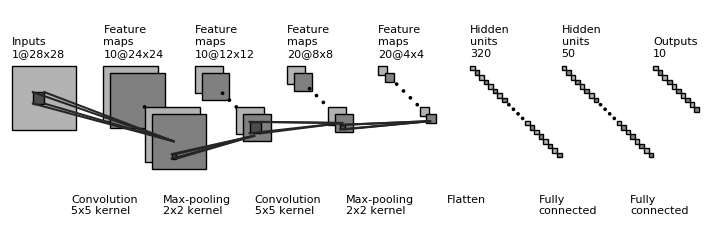
\includegraphics[width=0.9\linewidth]{figures/aistats19/conv.png}
    \caption{CNN architecture used for the MNIST experiments}
    \label{fig:arch}
\end{figure}

For REINFORCE, we use the same architecture as before. We train the model by sampling from the categorical distribution parameterized by the softmax output of the model and then computing a $\pm 1$ reward based on whether the model predicted the correct label. The loss function is the REINFORCE loss function given by,
\begin{equation}
    J(\theta) = \frac{1}{N} \sum_{i=1}^N r_i \log(\mathbb{P}(\hat y_i|x_i, \theta))
\end{equation}
where $\theta$ is the parameters of the model, $r_i$ is the reward obtained for example $i$, $\hat y_i$ is the predicted label for example $i$ and $x_i$ is the input feature vector for example $i$. The reward $r_i$ is given by $r_i = 2*\mathbb{I}[\hat y_i = y_i] - 1$, where $\mathbb{I}$ is the $0-1$ indicator function and $y_i$ is the true label for example $i$.

For ARS, we use the same architecture and reward function as before. The hyperparameters used are shown in Table \ref{tab:chosen-hyperparams} and we closely follow the algorithm outlined in \citep{mania2018simple}.

\paragraph{Linear Regression Experiments}
\label{sec:linreg-details}

We generate training and test data for the linear regression experiments as follows: we sampled a random $d+1$ dimensional vector $w$ where $d$ is the input dimensionality. We also sampled a random $d \times d$ covariance matrix $C$. The training and test dataset consists of $d+1$ vectors $x$ whose first element is always $1$ (for the bias term) and the rest of the $d$ terms are sampled from a multivariate normal distribution with mean $\mathbf{0}$ and covariance matrix $C$. The target vectors $y$ are computed as $y = w^Tx + \epsilon$ where $\epsilon$ is sampled from a univariate normal distribution with mean $0$ and standard deviation $0.001$.

We implemented both SGD and Newton Descent on the mean squared loss, for the supervised learning experiments. For SGD, we used a learning rate of $0.1$ for $d=10, 100$ and a learning rate of $0.01$ for $d=1000$, and a batch size of 64. For Newton Descent, we also used a batch size of 64. To frame it as a one-step MDP, we define a reward function $r$ which is equal to the negative of mean squared loss. Both REINFORCE and ARS use this reward function. To compute the REINFORCE loss, we take the prediction of the model $\hat{w}^Tx$, add a mean $0$ standard deviation $\beta = 0.5$ Gaussian noise to it, and compute the reward (negative mean squared loss) for the noise added prediction. The REINFORCE loss function is then given by
\begin{equation}
    J(w) = \frac{1}{N} \sum_{i=1}^N r_i \frac{- (y_i - \hat{w}^Tx_i)^2}{2\beta^2}
\end{equation}
where $r_i = -(y_i - \hat y_i)^2$, $\hat y_i$ is the noise added prediction and $\hat{w}^Tx_i$ is the prediction by the model. We use an Adam optimizer with learning rate and batch size as shown in Table \ref{tab:hyperparam-reinforce}. For the natural REINFORCE experiments, we estimate the fisher information matrix and compute the descent direction by solving the linear system of equations $Fx = g$ where $F$ is the fisher information matrix and $g$ is the REINFORCE gradient. We use SGD with a $O(1/\sqrt{T})$ learning rate, where $T$ is the number of batches seen, and batch size as shown in Table \ref{tab:hyperparam-nreinforce}.

For ARS, we closely follow the algorithm outlined in \citep{mania2018simple}.

\subsubsection{Multi-step Control Experiments}
\label{sec:multi-step-control-1}

\paragraph{Tuning Hyperparameters for ARS}
\label{sec:tuning-hyperp-ars}

We tune the hyperparameters for ARS \citep{mania2018simple} in both
mujoco and LQR experiments, similar to the one-step control
experiments. The candidate hyperparameter values are shown in Tables
\ref{tab:hyperparam-multi-ars-mujoco} and \ref{tab:hyperparam-multi-ars-lqr}. We have observed that using all the
directions in ARS is always preferable under the low horizon settings
that we explore. Hence, we do not conduct a hyperparameter search over
the number of top directions and instead keep it the same as the
number of directions.

\begin{table}[ht]
    \centering
    \begin{tabular}{|c|c|c|}
    \hline
    \textbf{Hyperparameter} & \textbf{Swimmer-v2} &
                                                    \textbf{HalfCheetah-v2}\\
    \hline
    Stepsize &  $0.03, 0.05, 0.08, 0.1, 0.15$ & $0.001, 0.003,
                                                0.005,0.008, 0.01$ \\
    \hline
    \# Directions &  $5, 10, 20$ & $5, 10, 20$\\
    \hline
    Perturbation & $0.05, 0.1, 0.15, 0.2$ & $0.01, 0.03, 0.05, 0.08$\\
    \hline
    \end{tabular}
    \caption{Candidate hyperparameters used for tuning in ARS experiments}
    \label{tab:hyperparam-multi-ars-mujoco}
\end{table}

\begin{table}[ht]
    \centering
    \begin{tabular}{|c|c|}
    \hline
    \textbf{Hyperparameter} & \textbf{LQR}\\
    \hline
    Stepsize &  $0.0001, 0.0003, 0.0005, 0.0008, 0.001, 0.003, 0.005,
               0.008, 0.01$ \\
    \hline
    \# Directions &  $10$ \\
    \hline
    Perturbation & $0.01, 0.05, 0.1$ \\
    \hline
    \end{tabular}
    \caption{Candidate hyperparameters used for tuning in ARS experiments}
    \label{tab:hyperparam-multi-ars-lqr}
  \end{table}

We use the hyperparameters shown in Tables
\ref{tab:chosen-hyperparam-multi-ars-swimmer} and \ref{tab:chosen-hyperparam-multi-ars-halfcheetah} chosen through tuning for each
of the multi-step experiments. The hyperparameters are chosen by
averaging the total reward obtained across three random seeds
(different from the 10 random seeds used in experiments presented in
Figure~\ref{fig:multistep}) and
chosing the setting that has the highest total reward after $10000$
episodes of training..

\begin{table}[ht]
    \centering
    \begin{tabular}{|c|c|c|c|}
    \hline
      \textbf{Horizon} & \textbf{Stepsize} &
                                             \textbf{\#
                                             Directions} &
                                                           \textbf{Perturbation}\\
      \hline
      $H = 1$ & 0.15  & 5  & 0.2 \\
      \hline
      $H = 2$ & 0.08  & 5 &  0.2\\
      \hline
      $H = 3$ & 0.15  & 5 &  0.2\\
      \hline
      $H = 4$ & 0.08  & 5 & 0.2 \\
      \hline
      $H = 5$ & 0.05  & 5 &  0.2\\
      \hline
      $H = 6$ & 0.08  &5  & 0.2 \\
      \hline
      $H = 7$ & 0.08  & 5 & 0.2 \\
      \hline
      $H = 8$ & 0.08  & 5 & 0.2 \\
      \hline
      $H = 9$ & 0.1  &5  & 0.2 \\
      \hline
      $H = 10$ & 0.08  &5  & 0.2 \\
      \hline
      $H = 11$ & 0.08  &5  & 0.2 \\
      \hline
      $H = 12$ & 0.1  &5  & 0.2 \\
      \hline
      $H = 13$ & 0.08  & 5 & 0.2 \\
      \hline
      $H = 14$ & 0.08  & 5 &0.2  \\
      \hline
      $H = 15$ & 0.08  & 10 & 0.2 \\
      \hline
    \end{tabular}
    \caption{Hyperparameters chosen for multi-step experiments for ARS
    in Swimmer-v2}
    \label{tab:chosen-hyperparam-multi-ars-swimmer}
\end{table}

\begin{table}[ht]
    \centering
    \begin{tabular}{|c|c|c|c|}
    \hline
      \textbf{Horizon} & \textbf{Stepsize} &
                                             \textbf{\#
                                             Directions} &
                                                           \textbf{Perturbation}\\
%0.001, 0.008, 0.008, 0.003, 0.003, 0.003, 0.008, 0.008, 0.01 ,
       %0.005, 0.008, 0.005, 0.008, 0.01 , 0.008
      \hline
      $H = 1$ & 0.001  & 20 & 0.08 \\
      \hline
      $H = 2$ & 0.008  & 5 &  0.08\\
      \hline
      $H = 3$ &  0.008  & 10 & 0.08 \\
      \hline
      $H = 4$ &  0.003  & 5 &  0.05\\
      \hline
      $H = 5$ &  0.003  & 5 &  0.05\\
      \hline
      $H = 6$ &  0.003  & 10 &  0.05\\
      \hline
      $H = 7$ &  0.008  & 20 &  0.05\\
      \hline
      $H = 8$ &  0.008  & 5 &  0.05\\
      \hline
      $H = 9$ &  0.01  & 20 &  0.03\\
      \hline
      $H = 10$ &   0.005 & 10 &  0.03\\
      \hline
      $H = 11$ &  0.008  & 20 &  0.03\\
      \hline
      $H = 12$ &  0.005  & 5 &  0.05\\
      \hline
      $H = 13$ &  0.008  & 20 &  0.03\\
      \hline
      $H = 14$ &  0.01  & 10 &  0.03\\
      \hline
      $H = 15$ &  0.008  & 20 &  0.03\\
      \hline
    \end{tabular}
    \caption{Hyperparameters chosen for multi-step experiments for ARS
    in HalfCheetah-v2}
    \label{tab:chosen-hyperparam-multi-ars-halfcheetah}
\end{table}


\paragraph{Tuning Hyperparameters for ExAct}
\label{sec:tuning-hyperp-exact}

We tune the hyperparameters for ExAct (Algorithm
\ref{alg:random_search_action}) in both mujoco and LQR experiments,
similar to ARS. The candidate hyperparameter values are shown in
Tables \ref{tab:hyperparam-multi-exact-mujoco} and
\ref{tab:hyperparam-multi-exact-lqr}. Similar to ARS, we do not
conduct a hyperparameter search over the number of top directions and
instead keep it the same as the number of directions.

\begin{table}[H]
    \centering
    \begin{tabular}{|c|c|c|}
    \hline
    \textbf{Hyperparameter} & \textbf{Swimmer-v2} &
                                                    \textbf{HalfCheetah-v2}\\
    \hline
    Stepsize &  $0.005, 0.008, 0.01, 0.015, 0.02, 0.025, 0.03$ & $0.0001, 0.0003,
                                                0.0005,0.0008, 0.001,
                                                                 0.002,
                                                                 0.003$ \\
    \hline
    \# Directions &  $5, 10, 20$ & $5, 10, 20$\\
    \hline
    Perturbation & $0.15, 0.2, 0.3, 0.5$ &  $0.15, 0.2, 0.3, 0.5$\\
    \hline
    \end{tabular}
    \caption{Candidate hyperparameters used for tuning in ExAct experiments}
    \label{tab:hyperparam-multi-exact-mujoco}
\end{table}

\begin{table}[ht]
  \centering
  \begin{tabular}{|c|c|}
    \hline
    \textbf{Hyperparameter} & \textbf{LQR}\\
    \hline
    Stepsize &  $0.0001, 0.0003, 0.0005, 0.0008, 0.001, 0.003, 0.005,
               0.008, 0.01$ \\
    \hline
    \# Directions &  $10$ \\
    \hline
    Perturbation & $0.01, 0.05, 0.1$ \\
    \hline
  \end{tabular}
  \caption{Candidate hyperparameters used for tuning in ExAct experiments}
  \label{tab:hyperparam-multi-exact-lqr}
\end{table}

We use the hyperparameters shown in Tables
\ref{tab:chosen-hyperparam-multi-exact-swimmer} and \ref{tab:chosen-hyperparam-multi-exact-halfcheetah} chosen through tuning for
each of the multi-step experiments, similar to ARS.

\begin{table}[ht]
    \centering
    \begin{tabular}{|c|c|c|c|}
    \hline
      \textbf{Horizon} & \textbf{Stepsize} &
                                             \textbf{\#
                                             Directions} &
                                                           \textbf{Perturbation}\\
      \hline
      $H = 1$ & 0.02  &5  & 0.2 \\
      \hline
      $H = 2$ & 0.02  & 5 & 0.2 \\
      \hline
      $H = 3$ & 0.015  & 10 & 0.2 \\
      \hline
      $H = 4$ & 0.015  & 10 & 0.2 \\
      \hline
      $H = 5$ & 0.01  & 10 & 0.2 \\
      \hline
      $H = 6$ & 0.015  & 10 & 0.2 \\
      \hline
      $H = 7$ & 0.01  & 20 & 0.2 \\
      \hline
      $H = 8$ & 0.015  & 20 & 0.2 \\
      \hline
      $H = 9$ & 0.02  & 20 & 0.2 \\
      \hline
      $H = 10$ & 0.008  & 5 & 0.2 \\
      \hline
      $H = 11$ & 0.02  & 5 & 0.15 \\
      \hline
      $H = 12$ & 0.02  & 20 & 0.2 \\
      \hline
      $H = 13$ & 0.015  & 5 & 0.15 \\
      \hline
      $H = 14$ & 0.02  & 10 &0.15  \\
      \hline
      $H = 15$ & 0.01  & 5 & 0.1 \\
      \hline
    \end{tabular}
    \caption{Hyperparameters chosen for multi-step experiments for ExAct
    in Swimmer-v2}
    \label{tab:chosen-hyperparam-multi-exact-swimmer}
\end{table}

\begin{table}[ht]
    \centering
    \begin{tabular}{|c|c|c|c|}
    \hline
      \textbf{Horizon} & \textbf{Stepsize} &
                                             \textbf{\#
                                             Directions} &
                                                           \textbf{Perturbation}\\

      \hline
      $H = 1$ &0.0001   &20  &  0.2\\
      \hline
      $H = 2$ &  0.001 & 5 &  0.2\\
      \hline
      $H = 3$ &  0.001  & 5 & 0.2\\
      \hline
      $H = 4$ &  0.001  & 5 & 0.2 \\
      \hline
      $H = 5$ &  0.001  &10  & 0.2 \\
      \hline
      $H = 6$ &  0.001  & 5 & 0.2 \\
      \hline
      $H = 7$ &  0.001  &10  & 0.2 \\
      \hline
      $H = 8$ &  0.001  & 5 & 0.2 \\
      \hline
      $H = 9$ &  0.001  & 5 & 0.2 \\
      \hline
      $H = 10$ &  0.001  & 5 & 0.2 \\
      \hline
      $H = 11$ & 0.0008   & 5 & 0.15 \\
      \hline
      $H = 12$ &  0.001  & 5 & 0.2\\
      \hline
      $H = 13$ &  0.001  & 10 & 0.2 \\
      \hline
      $H = 14$ &  0.001  & 5 & 0.2\\
      \hline
      $H = 15$ &  0.0008  & 10 & 0.2 \\
      \hline
    \end{tabular}
    \caption{Hyperparameters chosen for multi-step experiments for ExAct
    in HalfCheetah-v2}
    \label{tab:chosen-hyperparam-multi-exact-halfcheetah}
\end{table}


\paragraph{Mujoco Experiments}
\label{sec:mujoco-experiments}

For all the mujoco experiments, both ARS and ExAct use a linear
policy with the same number of parameters as the dimensionality of the
state space. The hyperparameters for both algorithms are chosen as
described above. Each algorithm is run on both
environments (Swimmer-v2
and HalfCheetah-v2) for $10000$ episodes of training across $10$
random seeds (different from the ones used for tuning). This is
repeated for each horizon value $H \in \{1, 2, \cdots, 15\}$. In each
experiment, we record the mean evaluation return obtained after
training and plot the results in Figure~\ref{fig:multistep}. For more details on the environments used, we
refer the reader to \citep{brockman2016openai}.

\paragraph{LQR Experiments}
\label{sec:lqr-experiments}

In the LQR experiments, we constructed a linear dynamical system
$x_{t+1} = Ax_t + Bu_t + \xi_t$ where $x_t \in \mathbb{R}^{100}$, $A \in \mathbb{R}^{100\times
  100}$, $B \in \mathbb{R}^{100}$, $u_t \in
\mathbb{R}$ and the noise $\xi_t \sim \mathcal{N}(0_{100}, cI_{100
  \times 100})$ with a small constant $c \in \mathbb{R}^+$. We
explicitly make sure that the maximum eigenvalue of $A$ is less than 1
to avoid instability. We fix a quadratic cost function $c(x, u) =
x^TQx + uRu$, where $Q = 10^{-3}I_{100 \times 100}$ and $R = 1$. The
hyperparameters chosen for both algorithms are chosen as described
above.

For each algorithm, we run it for noise covariance values $c \in
\{10^{-4}, 5\times 10^{-4}, 10^{-3}, 5\times 10^{-3}, 10^{-2}, 5\times 10^{-2},
10^{-1}, 5\times 10^{-1}\}$
until we reach a stationary point where $\|\nabla_\theta
J(\theta)\|_2^2 \leq 0.05$. The number of interactions with the
environment allowed is capped at $10^6$ steps for each run. This is
repeated across $10$ random seeds (different from the ones used for
tuning). The number of interactions needed to reach the stationary
point as the noise covariance is increased is recorded and shown in
Figure~\ref{fig:multistep}.


%%% Local Variables:
%%% mode: latex
%%% TeX-master: "../main"
%%% End:
